\documentclass[report.tex]{subfiles}

\begin{document}

\section{Vizualizácia konvergencie}\label{sec:EF}

Počas minimalizácie popísanej v predošlej sekcii sme taktiež ukladali body, cez ktoré metóda prechádzala. Ak označíme $J^*$ nájdené minimum danou metódou, môžeme vizualizovať euklidovskú normu rozdielu $J(x^k) - J^*$, kde $x^k$ je aproximácia minima v $k$-tej iterácii.

V nasledujúcich grafoch používame logaritmickú škálu na $y$-ovej osi, kde zobrazujeme $\lVert J(x^k) - J^*\rVert_2$. Na $x$-ovej je zobrazené poradové číslo iterácie. Bod $x^k$, v ktorom sa nadobúda hodnota $J^*$ nie je zahrnutý v grafe, keďže by sme ho nevedeli vyobraziť na logaritmickej osi.

\subsection{Vizualizácia konvergencie kvázinewtonovských metód}

Môžeme si všimnúť, že kvázinewtonovské metódy našli aproximáciu minima za menej ako 13 iterácií. Taktiež môžeme podľa tvaru lomenej čiary odhadovať kvadratickú konvergenciu metód, no graf s takýmto malým počtom vykreslených iterácií nepodáva dostatočnú informáciu na istejší odhad.

\begin{figure}[h!]
	\centering
	\begin{subfigure}[b]{0.4\linewidth}
		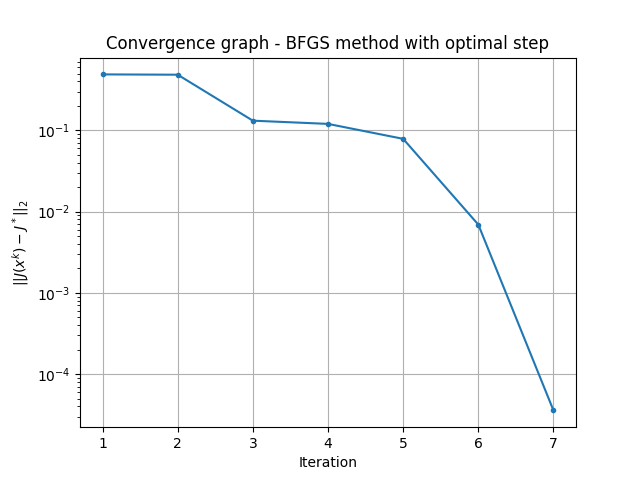
\includegraphics[width=\linewidth]{../../source/solvency_log_reg_results/BFGS_optimal.png}
		\caption{BFGS s optimálnym krokom}
	\end{subfigure}
	\begin{subfigure}[b]{0.4\linewidth}
		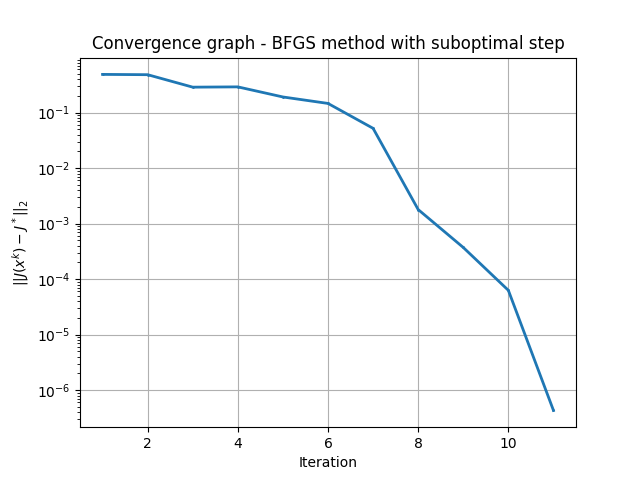
\includegraphics[width=\linewidth]{../../source/solvency_log_reg_results/BFGS_suboptimal.png}
		\caption{BFGS s približne optimálnym krokom}
	\end{subfigure}
	
	\begin{subfigure}[b]{0.4\linewidth}
		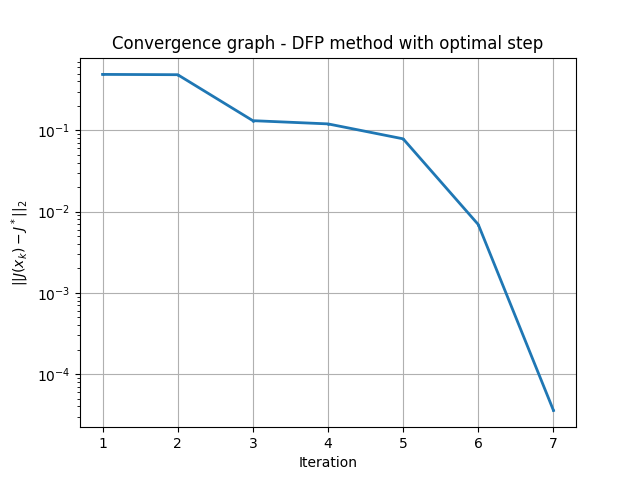
\includegraphics[width=\linewidth]{../../source/solvency_log_reg_results/DFP_optimal.png}
		\caption{DFP s optimálnym krokom}
	\end{subfigure}
	\begin{subfigure}[b]{0.4\linewidth}
		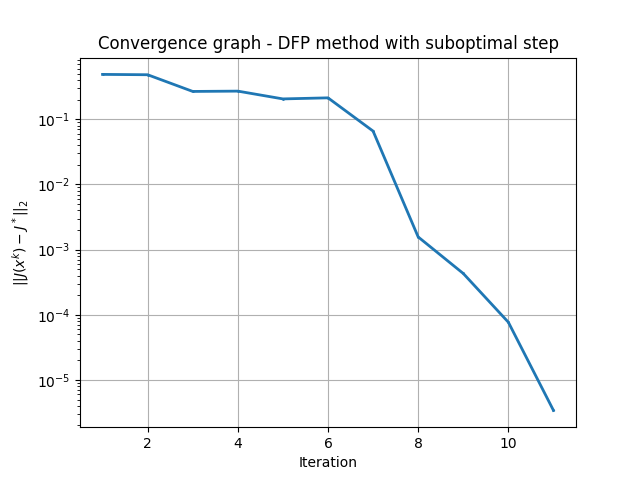
\includegraphics[width=\linewidth]{../../source/solvency_log_reg_results/DFP_suboptimal.png}
		\caption{DFP s približne optimálnym krokom}
	\end{subfigure}
	\label{fig:quasinewton}
\end{figure}

\newpage

\subsection{Vizualizácia konvergencie gradientných metód}

Vidíme, že pri gradientných metódach je počet iterácií na nájdenie aproximácie minima rádovo vyšší (ako bolo spomenuté, gradientná metóda s konštantným krokom po 10000 iteráciách nenašla aproximáciu minima takú, ktorá by spĺňala kritérium optimality). Taktiež z grafov môžeme odhadnúť, že väčšiu časť minimalizácie konvergovali k optimu lineárne.

\begin{figure}[h!]
	\centering
	\begin{subfigure}[b]{0.4\linewidth}
		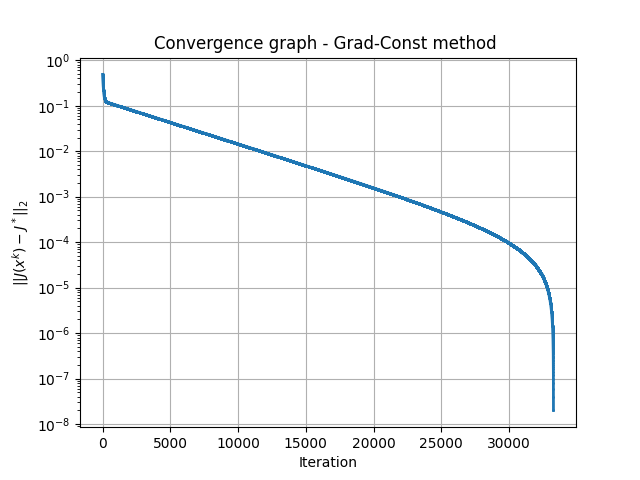
\includegraphics[width=\linewidth]{../../source/solvency_log_reg_results/Grad-Const.png}
		\caption{konštantný krok}
	\end{subfigure}
	\begin{subfigure}[b]{0.4\linewidth}
		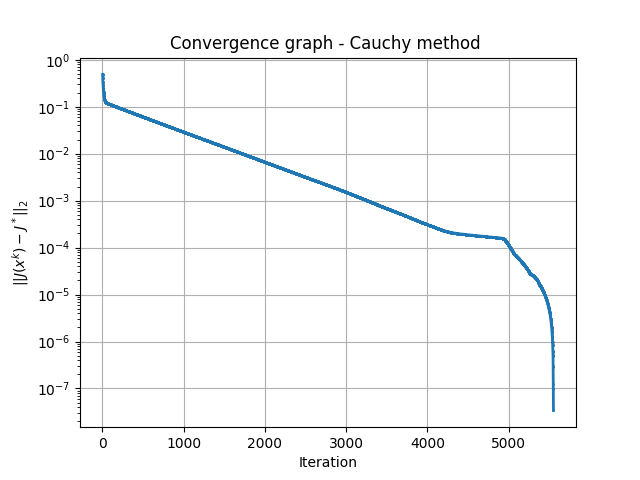
\includegraphics[width=\linewidth]{../../source/solvency_log_reg_results/Cauchy.png}
		\caption{optimálny krok}
	\end{subfigure}
	\label{fig:gradient}
\end{figure}

\end{document}  